\section{Sequential Exploration: Explore Early, Exploit Late}
\label{sec:exploitation-vs-exploration}
% YCH: "exploration" is a specific term in RL, while "effective exploration" is not. 
Exploration is a cornerstone of reinforcement learning, enabling agents to discover high-quality policies rather than settling on suboptimal solutions~\citep{sutton1998reinforcement, ladosz2022exploration}. 
%
This principle becomes particularly vital in deep RL, where vast action spaces render exhaustive search infeasible.
% This principle is especially critical in deep RL, where vast action spaces make exhaustive search intractable. 
%
% \begin{figure}[t!]
% % \begin{wrapfigure}{r}{0.6\textwidth}
% \begin{subfigure}[t]{0.4\textwidth}
% \centering
%      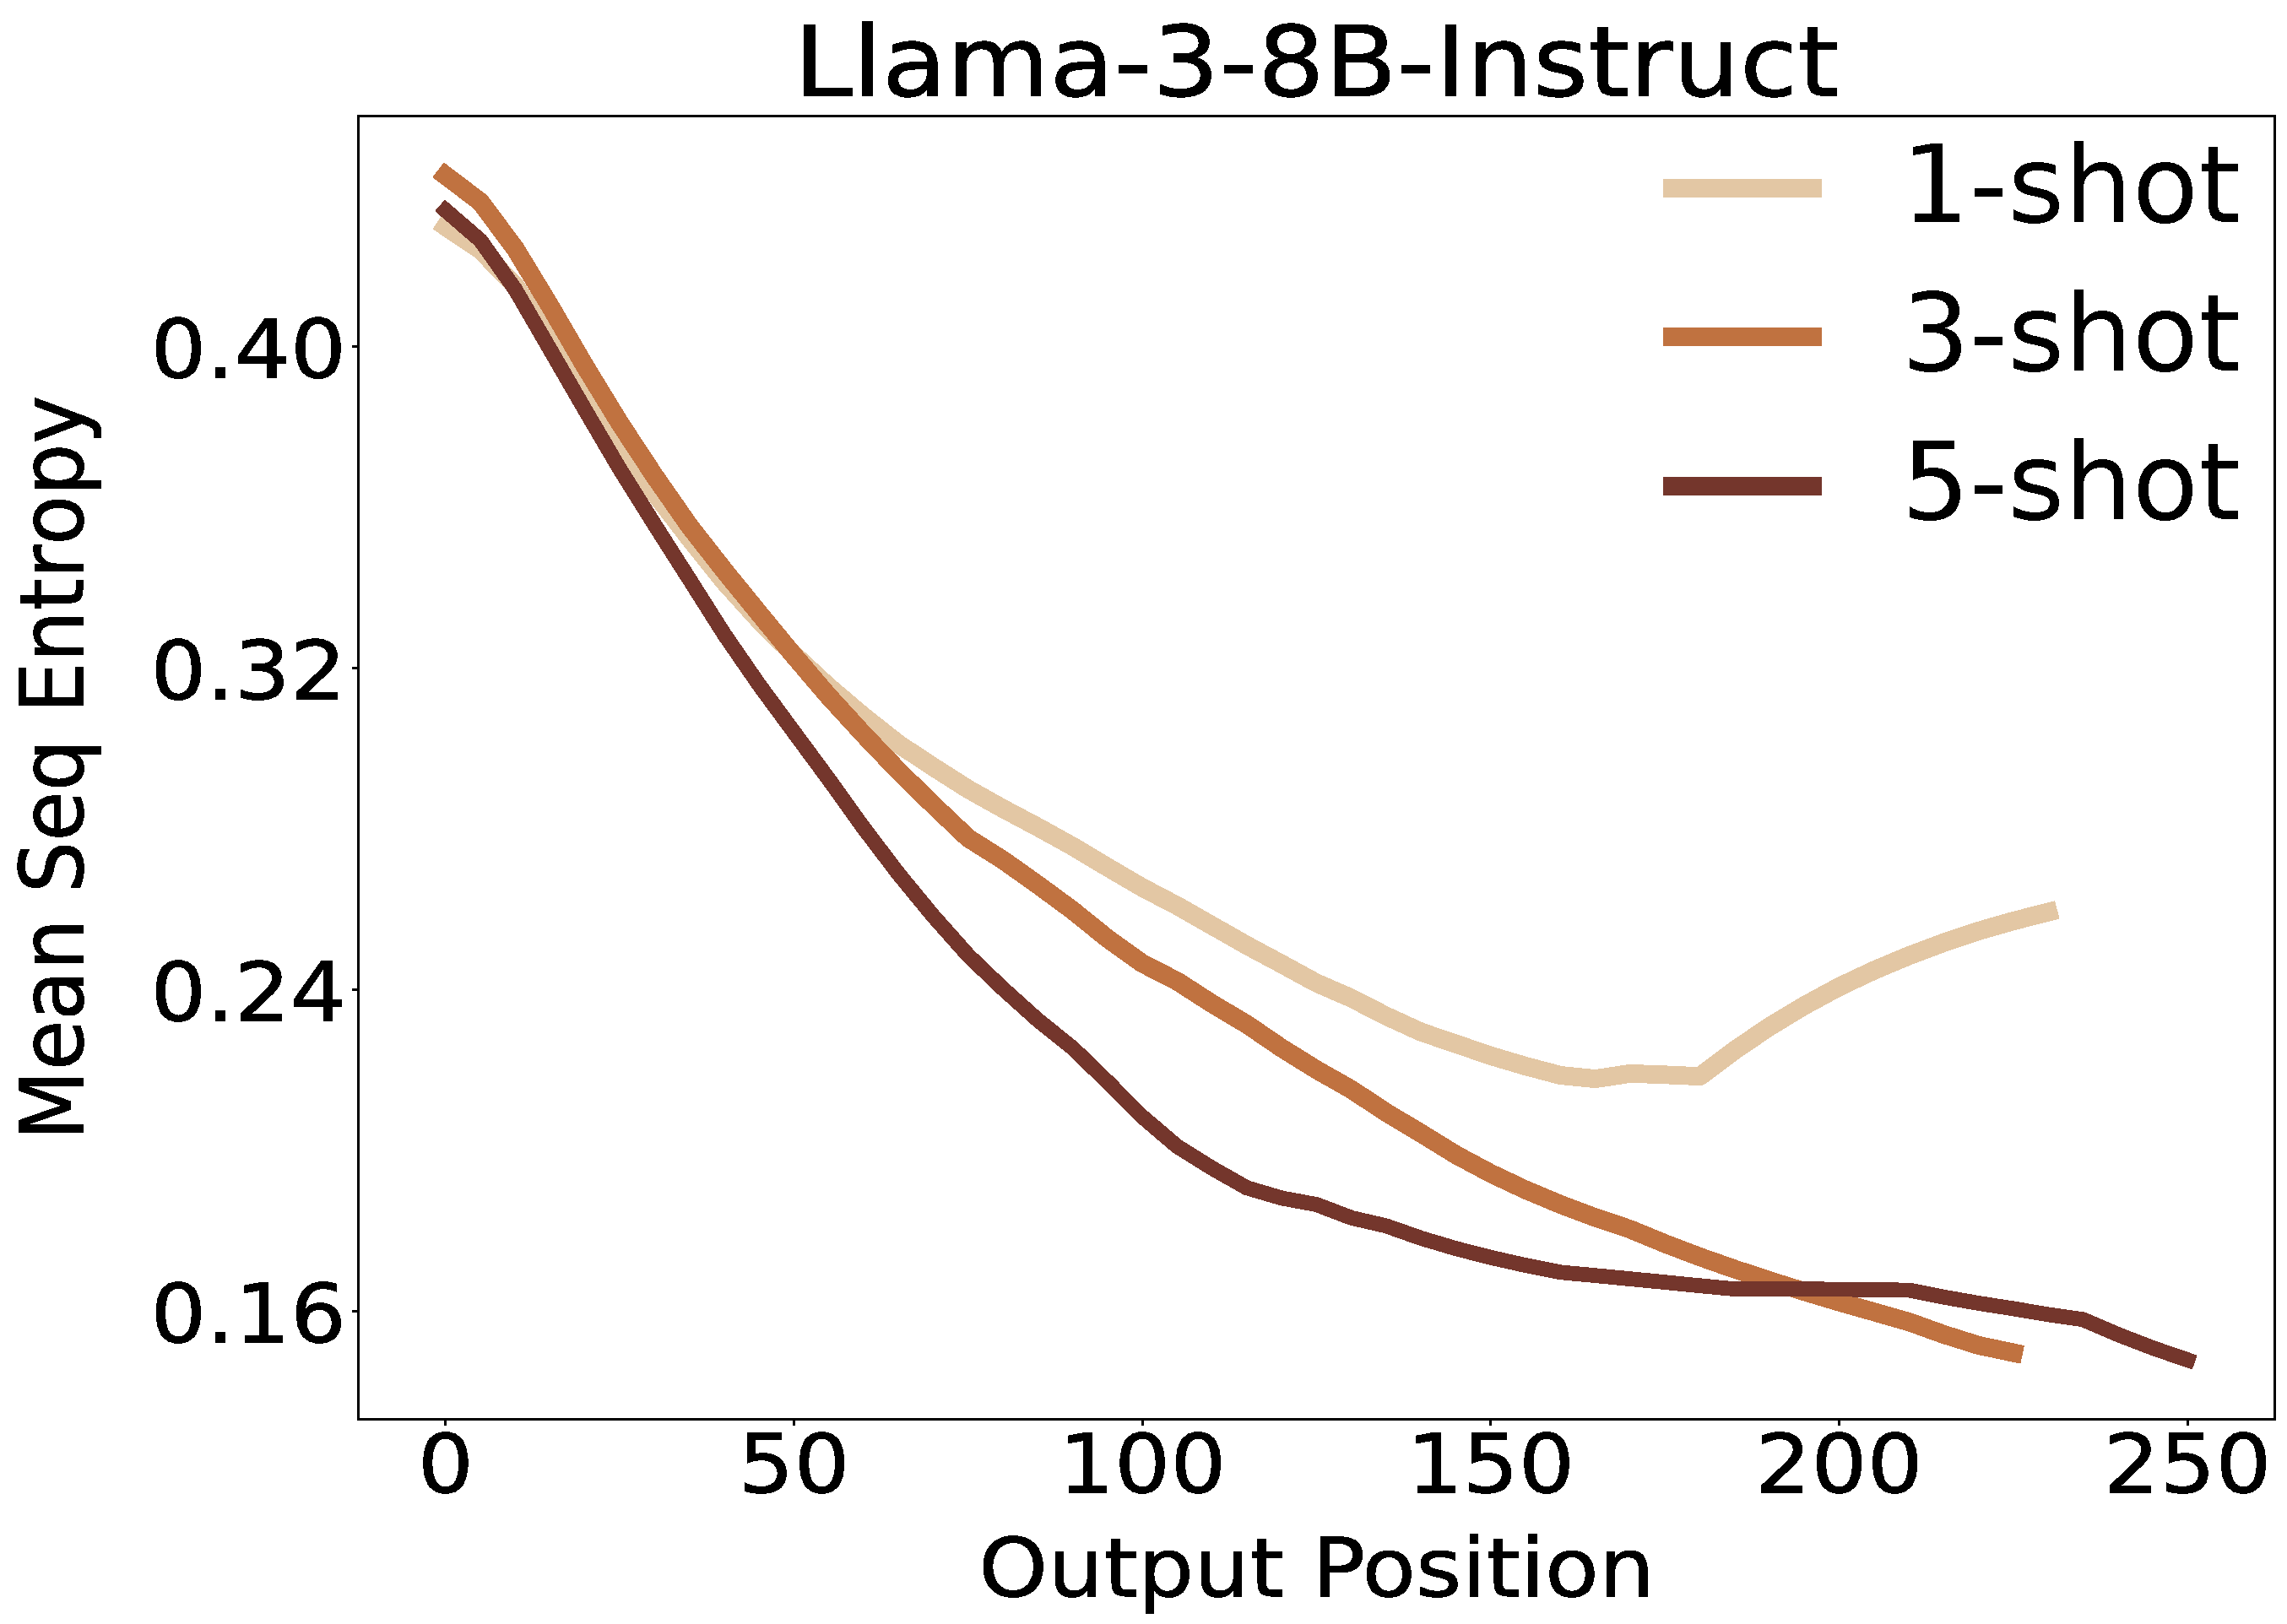
\includegraphics[width=\linewidth]{iclr2026/figures/branching_factor_figure/piecewise_ebf_Llama-3-8B-Instruct_mean_seq_entropy_fixed_start.pdf}
%      \caption{}
%     \label{fig: entropy_sequential_dynamic}
% \end{subfigure}
% \begin{subfigure}[t]{0.6\textwidth}
%     \centering
%     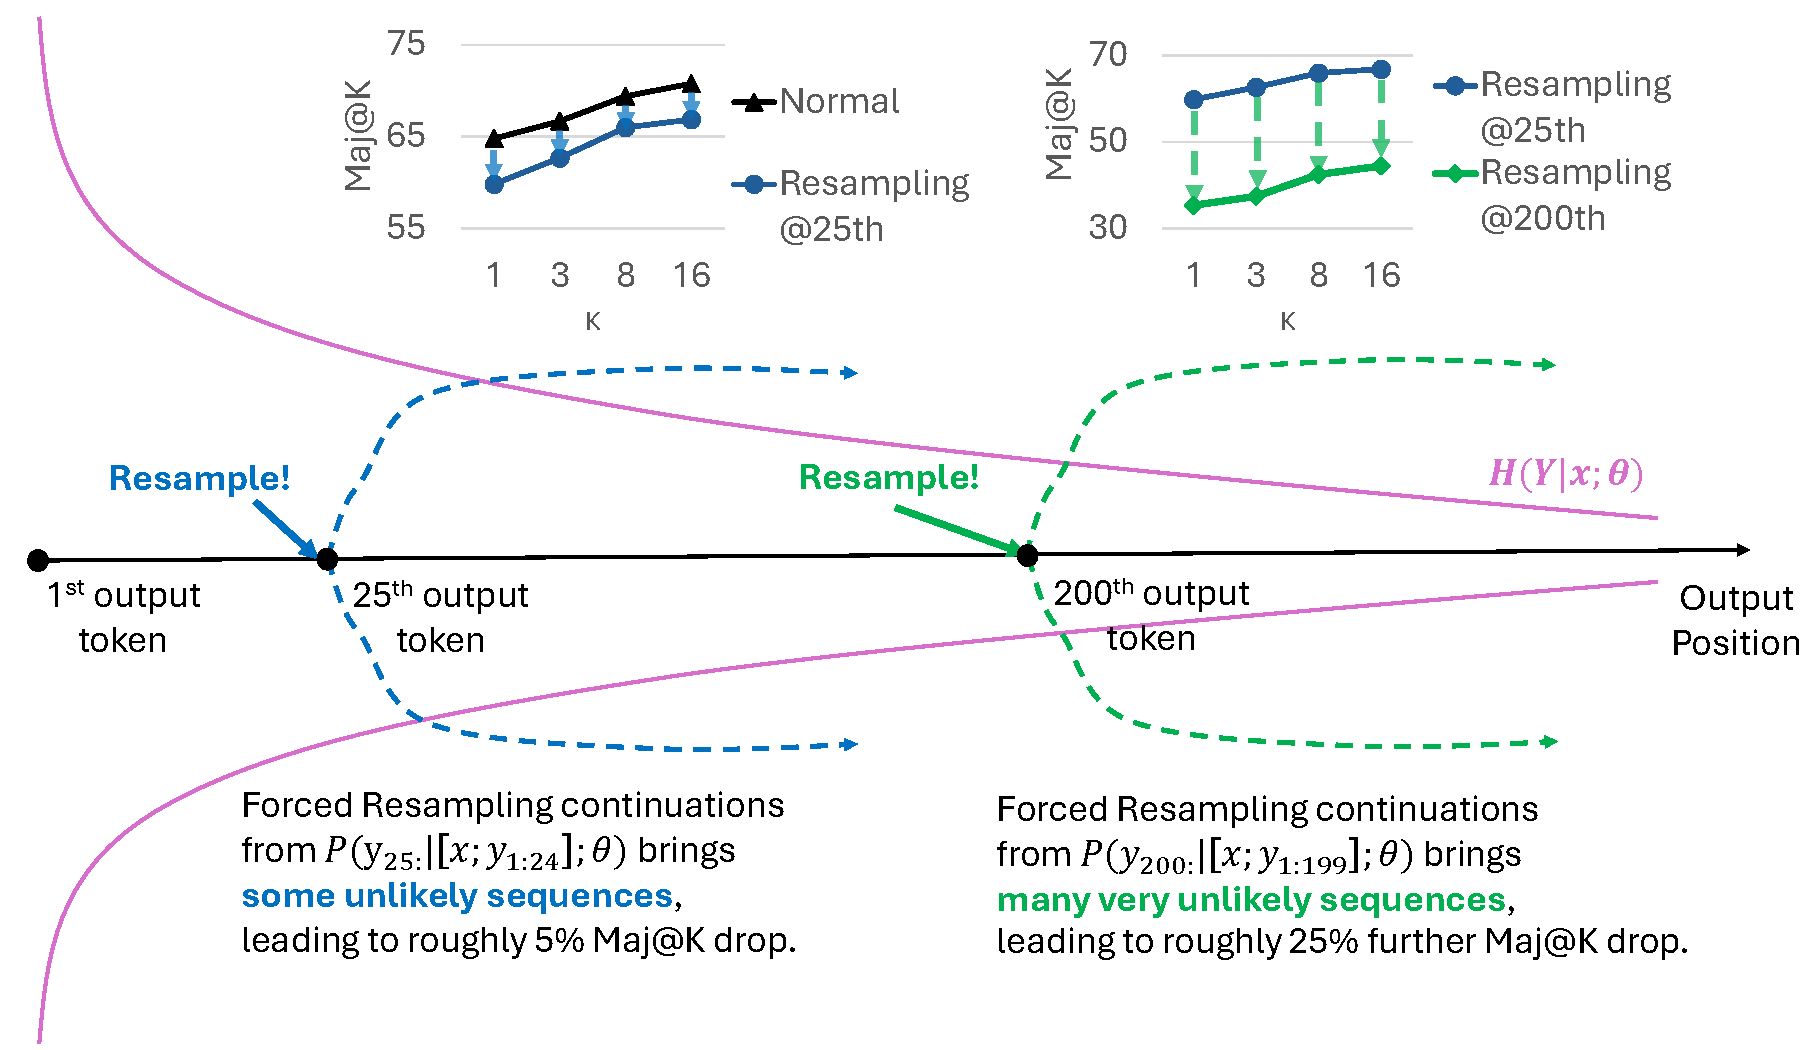
\includegraphics[width=\linewidth]{iclr2026/figures/branching_factor_figure/bon_from_middle_demo.pdf}    
%     \caption{}
%     \label{fig:forking_experiment}
% \end{subfigure}
% \caption{
%     (a): Average entropy shrinks with output positions for Llama-3-8B-Instruct on MMLU dataset. (b): A ``forking'' experiment on DeepSeek-Distilled Llama-3 shows early branching (high-entropy region) yields higher Maj@k on MMLU than late branching (low-entropy region).
% }
% \vspace{-10pt}
% % \end{wrapfigure}
% \end{figure}
%
% YCH: I insist on using "manifests as" rather than using "cause" -- this is most accurate description based on how these literature presents it. They do not consistently say explicitly that insufficient exploration lead to sth, not to mention establishing a strict causal relation. Instead they are showing this phenomenon and derive some entropy-promoting methods (forking tokens, kl-clip, etc). 
% YCH: anyway the entropy would reduce as the training goes sufficiently long (otherwise I guess the convergence properties would be fairly brittle), regardless of what exploration strategies we are using. It is just a matter of whether we want to see it early or later. 
In the context of RL for language models (e.g., RLVR), insufficient exploration often manifests as  \textit{entropy collapse}, i.e., a premature narrowing of the generation distribution during training~\citep{yu2025dapo, wang2025beyond, cui2025entropy}.
% 
% YCH: I do not feel this context is ready (e.g., "diversity" concept is not introduced previously), also I do not think we want to rigorously claim that "exploration-exploitation trade-off" is "tied to" "quality-diversity trade-off" -- we really do not have that proof anywhere to be honest. Also temperature sampling is not invented to achieve "Q-D trade-off" -- it is used in MaxEntRL more to achieve "E-E trade-off". 
% So I would suggest we tone down and get back to original way 
% Since exploration and exploitation are closely tied to the diversity and quality of generated outputs during training,
% YCH: A ... way to...is ... **through [ABCD]** this is not grammatically correct, or at least not used often. "Through [ABCD]" could not be used as an object in the S-V-O structure.  
A common simple tool to encourage exploration is \emph{temperature sampling}.
% 
However, a \textit{fixed} temperature imposes a difficult trade-off. 
%
% YCH: "incoherence" does not necessarily mean "non-sensical tokens" -- sure, non-sensical tokens would break the flow and impact coherence, but incoherence can involve a bunch of reasonable tokens but still reads weird (e.g., transitioning between unrelated topics). If we can say it clearly following the literature, we should do that. 
A high temperature promotes diversity (as indicated by increased entropy\footnote{See \cref{app:entropy_proof} for the proof.}), but it risks degrading output quality with nonsensical tokens and hallucinations~\citep{renze-2024-effect, wang2025beyond}. 
%
In contrast, a low temperature limits the discovery of novel solutions, leading to generic and repetitive outputs~\citep{Holtzman2020The, guo2025deepseek}.
%
\begin{wrapfigure}{r}{0.3\textwidth}
\vspace{-0.25in}
    \centering
    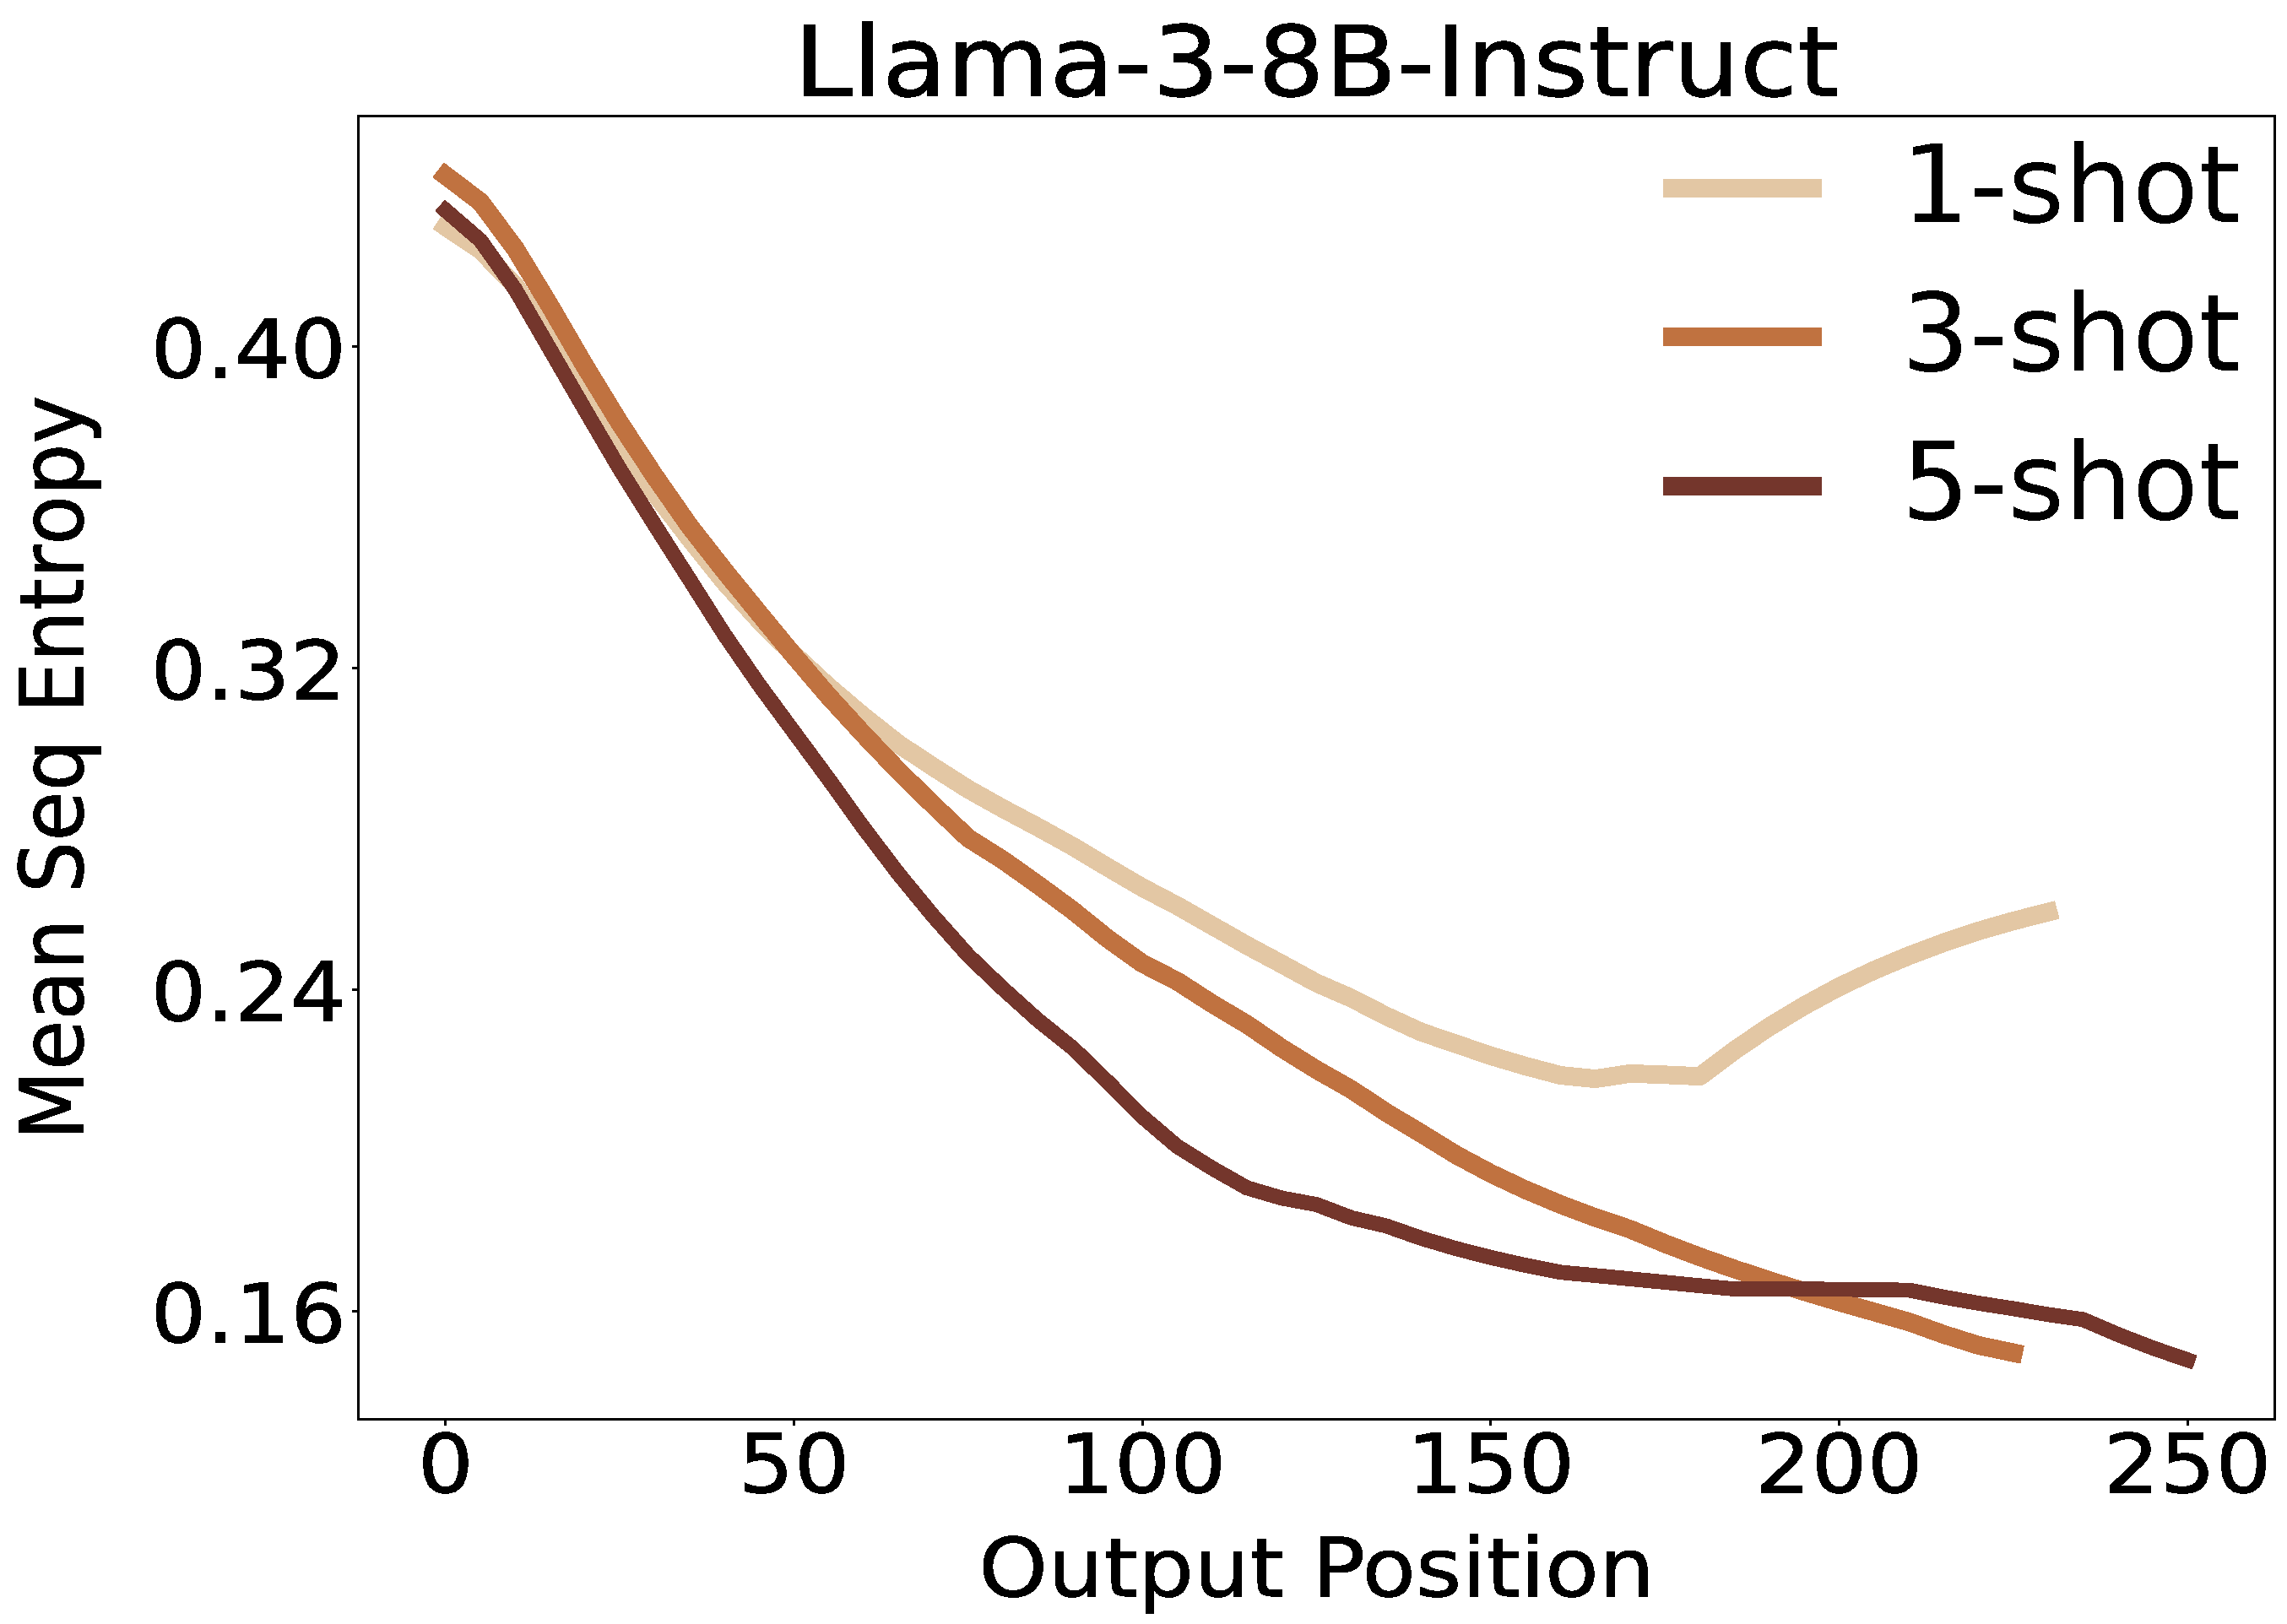
\includegraphics[width=\linewidth]{iclr2026/figures/branching_factor_figure/piecewise_ebf_Llama-3-8B-Instruct_mean_seq_entropy_fixed_start.pdf}
    \vspace{-0.3in}
    \caption{
    Average entropy shrinks with output positions for Llama-3-8B-Instruct on MMLU dataset. 
    }
    % \vspace{-0.2in}
    \label{fig: entropy_sequential_dynamic}
\end{wrapfigure}
%
The key to resolving this dilemma lies not in finding a single best temperature, but in recognizing that exploration requirements vary throughout the generation process.
% 
This key insight stems directly from the autoregressive nature of language models.
% \zz{don't feel like this worth to be bold?}
%
At the beginning of a sequence, the context is minimal and uncertainty is high, allowing a wide range of valid continuations. 
%
% YCH: I feel "the context narrows" reads weird? But I am okay with that. 
As more tokens are produced, the context becomes increasingly specific, constraining subsequent choices.
% As the model generates more tokens, the context becomes increasingly specific, constraining future choices. 
%
%
\revise{We reference the Data Processing Inequality (DPI)~\citep{shannon1948mathematical} as a \textit{theoretical motivation} to investigate these entropy dynamics. While not a strict derivation for autoregressive models, the DPI provides a framework to hypothesize that expected conditional entropy tends to decrease as the context grows}\footnote{While specific rollouts may have late high-entropy positions, the probability of this is exponentially small with position $t$~\citep{yang2025alignment}, making the overall trend a reliable heuristic.}:
% This intuition is supported by information theory: the data processing inequality~\citep{shannon1948mathematical} states that expected conditional entropy tends to decrease with each step
% \footnote{While specific rollouts may have late high-entropy positions, the probability of this is exponentially small with position $t$~\citep{yang2025alignment}, making the overall trend a reliable heuristic.}:
% This natural uncertainty reduction is formalized by the data processing inequality~\citep{shannon1948mathematical}, which shows that expected conditional entropy tends to decrease with each step\footnote{While specific rollouts may have late high-entropy positions, the probability of this is exponentially small with position $t$~\citep{yang2025alignment}, making the overall trend a reliable heuristic.}:
%
% \vspace{0.2in}
\begin{small}
\begin{align}
\label{eq:entropy_decay}
H(Y_t | [x, Y_{<t}]; \theta) &= \underbrace{\mathbb{E}_{y_{<t}}\big[ H(Y_t | [x, y_{<t}]; \theta) \big]}_{\substack{\text{Expected entropy at step } t \\ \text{(average over all prefixes } y_{<t}\text{)}}} 
\geq 
\underbrace{\mathbb{E}_{y_{<t+1}}\big[ H(Y_{t+1} | [x, y_{<t+1}]; \theta) \big]}_{\substack{\text{Expected entropy at step } t+1 \\ \text{(average over all prefixes } y_{<t+1}\text{)}}} = H(Y_{t+1} | [x, Y_{<t+1}]; \theta)\nonumber
% \vspace{0.2in}
\end{align}
\end{small}We further validate this empirically by examining position-wise entropy trend on the MMLU dataset~\citep{hendrycks2021measuring}\footnote{We use MMLU as a held-out dataset with Chain-of-Thought prompting~\citep{wei2022chain} to incentivize longer reasoning outputs, aligning with a typical RLVR scenario.} with Llama-3-8B-Instruct~\citep{grattafiori2024llama} (see \cref{fig: entropy_sequential_dynamic}).
% \vspace{0.2in}
% \footnote{The conditional entropy at step $t$ is an expectation over the distribution of all possible prefixes generated up to that point: $H(Y_t | [X, Y_{<t}]) = \mathbb{E}_{y_{<t} \sim P(Y_{<t}|X)} H(Y_t | [X, y_{<t}])$.}
%
% We provide an empirical verification of position-wise entropy trend on MMLU~\citep{hendrycks2021measuring} dataset in \cref{fig: entropy_sequential_dynamic} with \textsc{Llama-3-8B-Instruct}. 
% \begin{wrapfigure}{r}{0.45\textwidth}
% \vspace{-0.15in}
%     \centering
%     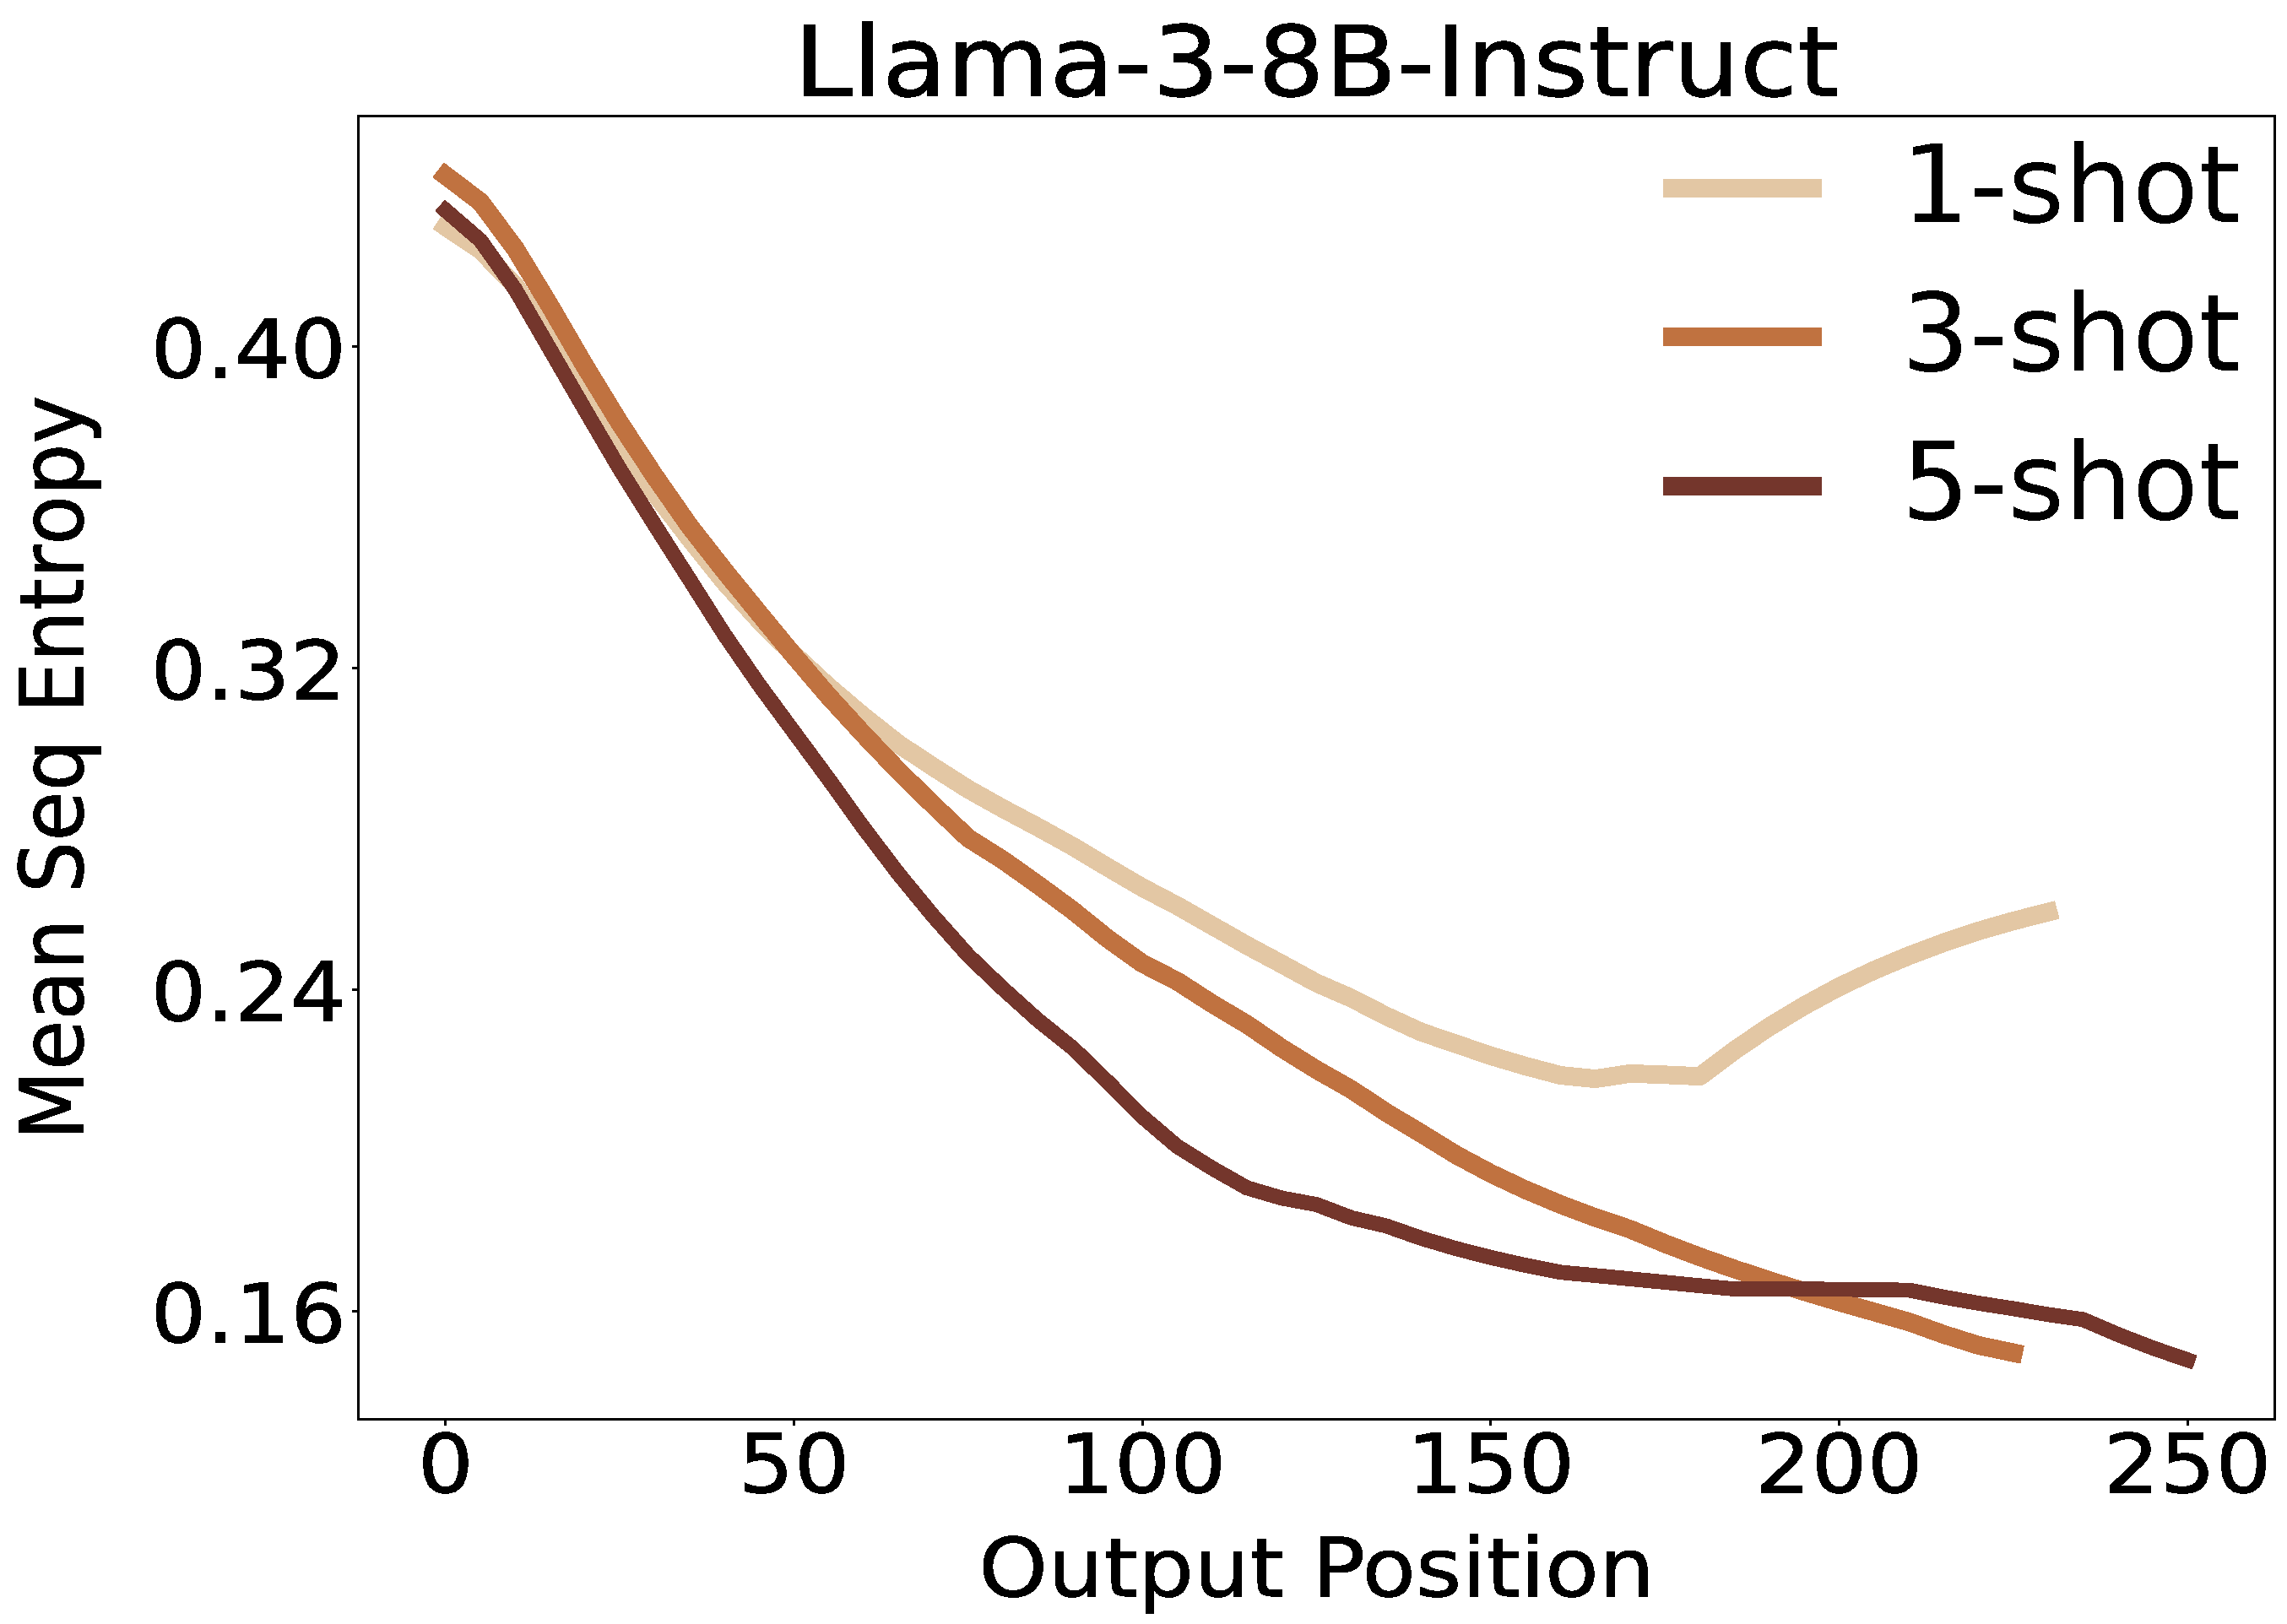
\includegraphics[width=\linewidth]{iclr2026/figures/branching_factor_figure/piecewise_ebf_Llama-3-8B-Instruct_mean_seq_entropy_fixed_start.pdf}
%     \vspace{-5mm}
%     \caption{
%     Average entropy shrinks with output positions for Llama-3-8B-Instruct on MMLU dataset.
%     % \zz{Nit (nitpick): 1. make the lines the same color, with more shots line ``darker" in color; 2. make the legends  (1-shot, 3-shot, 5-shot) bigger}
%     }
%     \vspace{-0.05in}
%     \label{fig: entropy_sequential_dynamic}
% \end{wrapfigure}
%
% We empirically validate this position-wise entropy trend on the MMLU dataset~\citep{hendrycks2021measuring}\footnote{We use MMLU as a held-out dataset with Chain-of-Thought prompting~\citep{wei2022chain} to incentivize the model to generate longer reasoning outputs to align with a typical RLVR scenario. } using Llama-3-8B-Instruct~\citep{grattafiori2024llama}, as illustrated in \cref{fig: entropy_sequential_dynamic}.


% \begin{wrapfigure}{r}{0.45\textwidth}
% \vspace{-0.2in}
%     \centering
%     \includegraphics[width=\linewidth]{iclr2026/figures/your_teaser_figure_path.pdf}
%     \vspace{-5mm}
%     \caption{A ``forking'' experiment on DeepSeek-Distilled Llama-3 shows early branching (high-entropy region) yields higher Maj@k on MMLU than late branching (low-entropy region).}
%     \vspace{-0.15in}
%     \label{fig:forking_experiment}
% \end{wrapfigure}
% \begin{wrapfigure}{r}{0.6\textwidth}
%     \centering
%     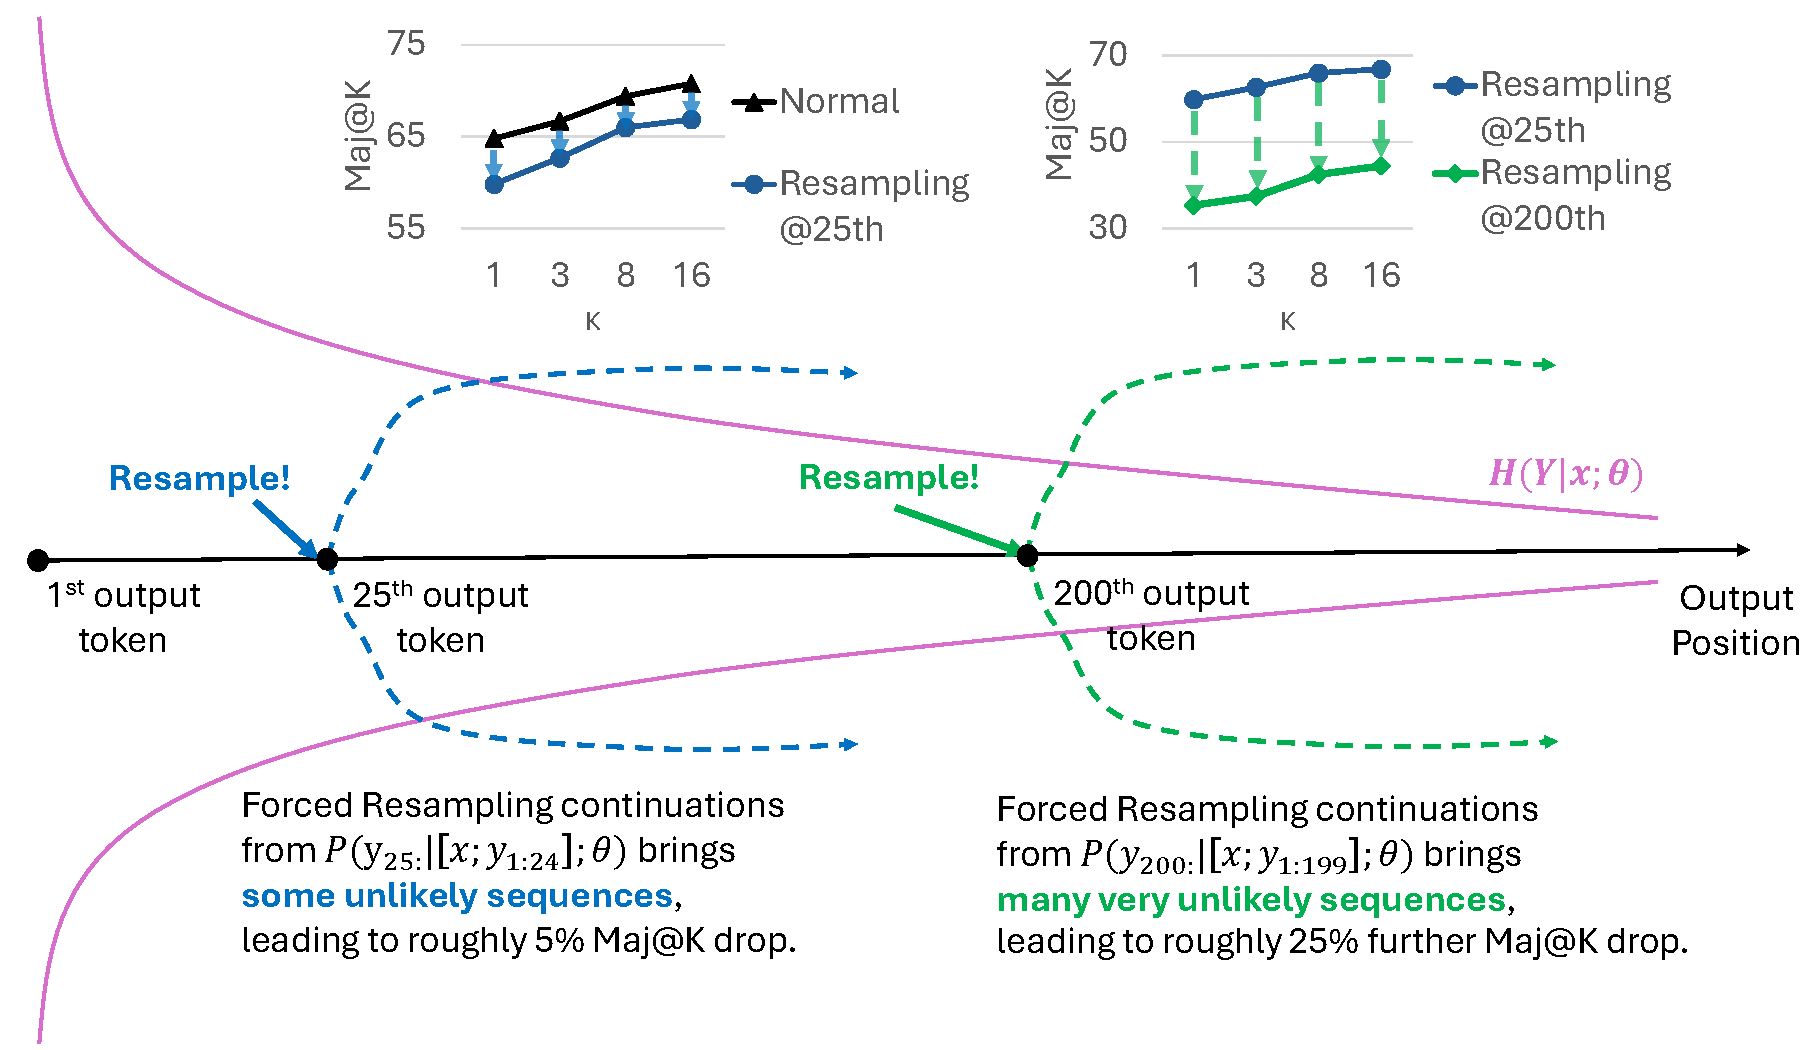
\includegraphics[width=\linewidth]{iclr2026/figures/branching_factor_figure/bon_from_middle_demo.pdf}    
% \caption{
%     A ``forking'' experiment on DeepSeek-Distilled Llama-3 shows early branching (high-entropy region) yields higher Maj@k on MMLU than late branching (low-entropy region).
% }
% \label{fig:forking_experiment}
% \end{wrapfigure}
\begin{wrapfigure}{r}{0.6\textwidth}
\vspace{-0.15in}
    \centering
    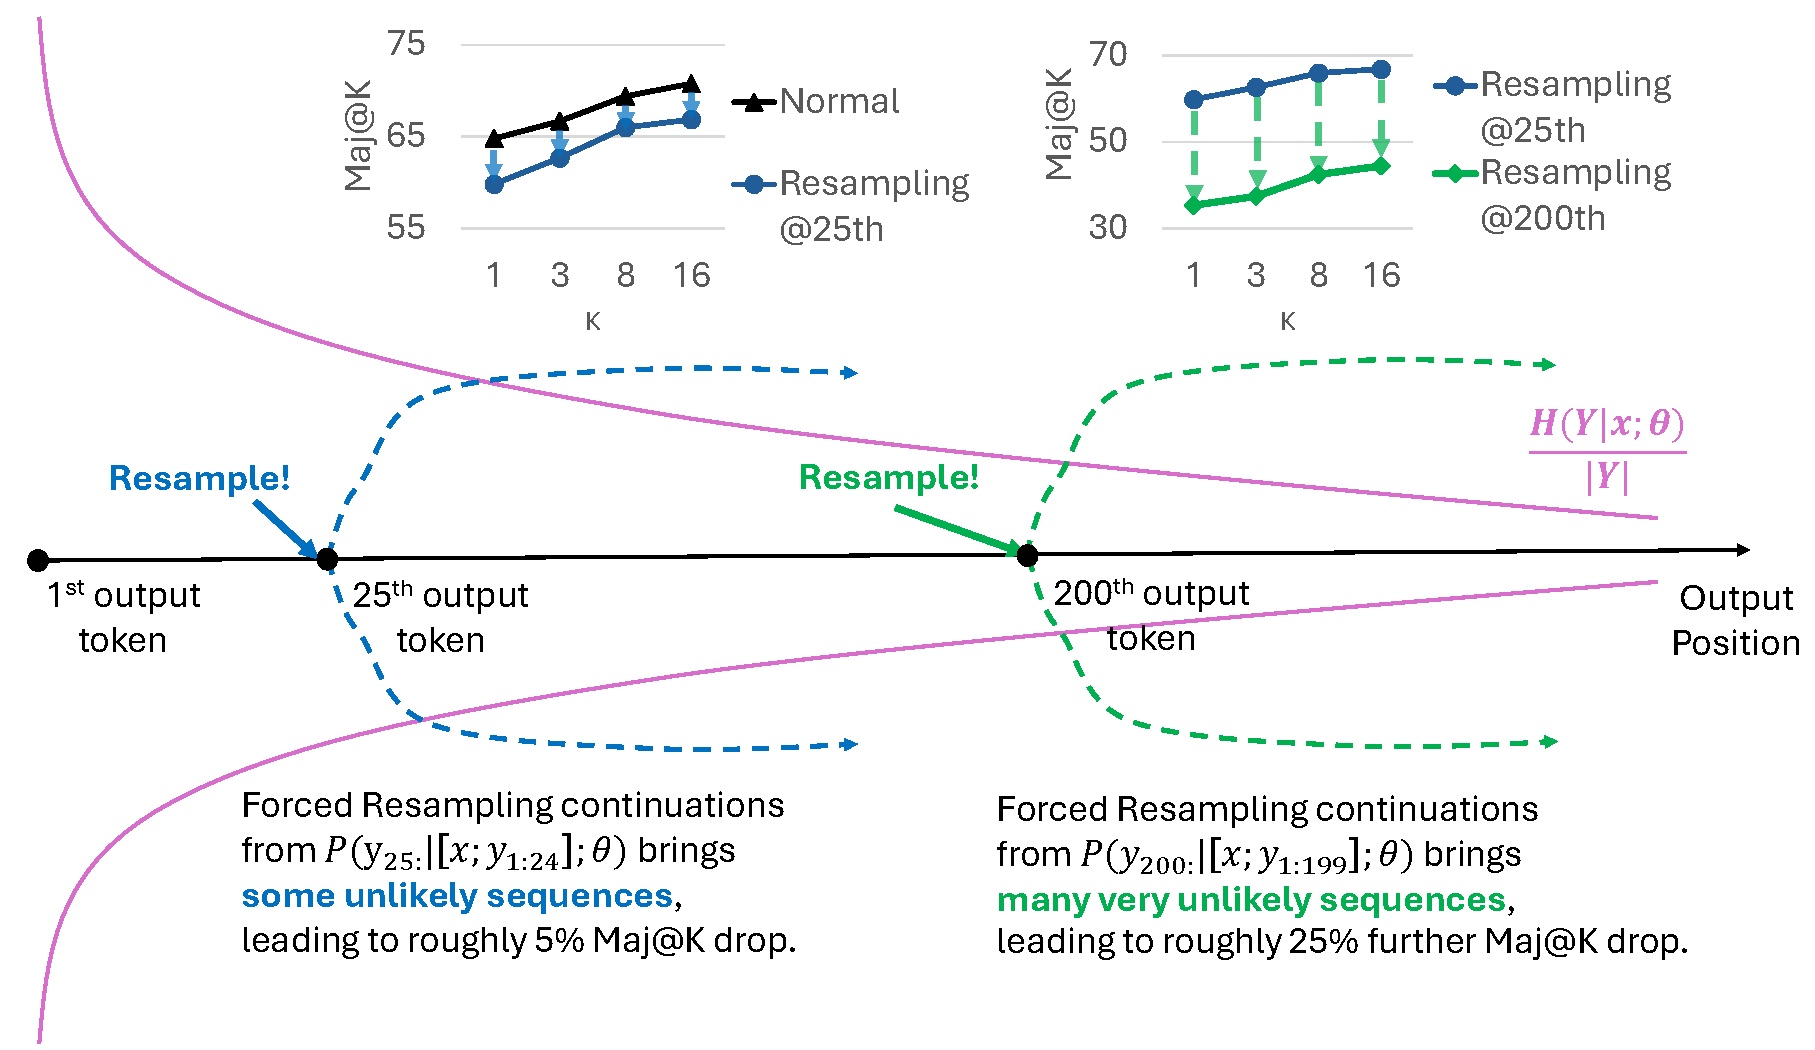
\includegraphics[width=\linewidth]{iclr2026/figures/branching_factor_figure/bon_from_middle_demo_v2.pdf}
    \vspace{-0.1in}
    \caption{
       A ``forking'' experiment on DeepSeek-Llama-3 shows early branching (high-entropy region) yields higher Maj@$k$ on MMLU than late branching (low-entropy region).
    }
\label{fig:forking_experiment}
\vspace{-0.05in}
\end{wrapfigure}
%
% YCH: Again I personally do not want to see hyphens that often -- I doubt people would use it to detect whether this is generated by chatgpt. 
This entropy decay has a direct performance implication: effective exploration, producing diverse, high-quality responses, is most beneficial in an uncertain, high-entropy phase at the start of generation.
%
To verify this, we replicate a controlled ``forking'' experiment~\citep{yang2025alignment} on DeepSeek-Distilled Llama-3-8B~\citep{guo2025deepseek}, a representative RLVR-fine-tuned model from the same Llama-3 family. 
%
As shown in \cref{fig:forking_experiment}, trajectories branched from early generation steps consistently outperform those branched later. 
%
% YCH: "align/aligning" should not occur that often in the near context -- it is again stylistically weak.  
This finding is also consistent with observations from inference-time analysis, where forced, late-stage exploration tends to degrade output quality~\citep{liao2025lost, yang2025alignment, fu2025deep}.
%

% I think mentioning classic results is redundant here.
% These converging lines of evidence provide a clear guide for applying a classic RL principle: agents should increase exploration in states of high uncertainty~\citep{ziebart2008maximum, schulman2017equivalence, haarnoja2018soft}. 
%
Aligning our strategy with the natural dynamics of generation, we arrive at a simple yet powerful design principle: \textbf{explore early and exploit late}.

%

% This position-dependent entropy curve provides a clear guide for applying a classic RL principle: agents should increase exploration in states of high uncertainty~\citep{ziebart2008maximum, schulman2017equivalence, haarnoja2018soft}. 
% %
% By aligning our strategy with the natural dynamics of generation, we arrive at a simple yet powerful design principle: \textbf{explore early and exploit late}. 
% %
% This involves encouraging strong exploration when the generative trajectory is wide, and gradually shifting toward exploitation as it narrows. 
% %
% In the next section, we will introduce a concrete method that instantiates this principle.
%
% The key to resolving this dilemma lies not in finding a single best temperature, but in recognizing that the need for exploration changes throughout the generation process. This insight stems directly from the autoregressive nature of language models, where the expected conditional entropy tends to decrease with each step (see \cref{eq:entropy_decay}). We empirically demonstrate that this entropy decay is a robust phenomenon across different types of models in \cref{fig:entropy_comparison}. The trend holds for a general-purpose instruct model (\cref{fig:entropy_instruct}) and is equally prominent in a state-of-the-art reasoning model fine-tuned with RLVR-style distillation (\cref{fig:entropy_rlvr}).

% \section{Sequential Exploration: Explore Early, Exploit Late}
% \label{sec:exploitation-vs-exploration}
% Exploration is a cornerstone of RL, enabling agents to discover effective policies and avoid converging to suboptimal solutions~\citep{sutton1998reinforcement, ladosz2022exploration}. This principle is especially critical in deep RL, where vast action spaces make exhaustive search intractable. In the context of RLVR, insufficient exploration often manifests as \textit{entropy collapse}---a premature narrowing of the generation distribution~\citep{yu2025dapo, wang2025beyond, cui2025entropy}. A common tool to encourage exploration is temperature sampling; however, a \textit{fixed} temperature imposes a difficult trade-off. A high temperature promotes diversity but risks introducing nonsensical outputs late in the generation process~\citep{renze-2024-effect, wang2025beyond}, while a low temperature limits the discovery of novel solutions~\citep{Holtzman2020The, guo2025deepseek}.

% The key to resolving this dilemma lies not in finding a single best temperature, but in recognizing that the need for exploration changes throughout the generation process. This insight stems directly from the autoregressive nature of language models. At the beginning of a sequence, the context is minimal and uncertainty is high. As the model generates more tokens, the context becomes increasingly specific, constraining future choices. This natural uncertainty reduction is formalized by the data processing inequality, which shows that expected conditional entropy tends to decrease with each step:\footnote{While specific rollouts may have late high-entropy positions, the probability of this will decay quickly with position $t$~\citep{yang2025alignment}, making the overall trend a reliable heuristic.}
% \begin{equation}
% \label{eq:entropy_decay}
% H(Y_t | [x, Y_{<t}]) = \underbrace{\mathbb{E}_{y_{<t}}\big[ H(Y_t | [x, y_{<t}]) \big]}_{\substack{\text{Expected entropy at step } t}}
% \geq 
% \underbrace{\mathbb{E}_{y_{<t+1}}\big[ H(Y_{t+1} | [x, y_{<t+1}]) \big]}_{\substack{\text{Expected entropy at step } t+1}} = H(Y_{t+1} | [x, Y_{<t+1}])\nonumber
% \end{equation}
% \begin{wrapfigure}{r}{0.45\textwidth}
% \vspace{-0.15in}
%     \centering
%     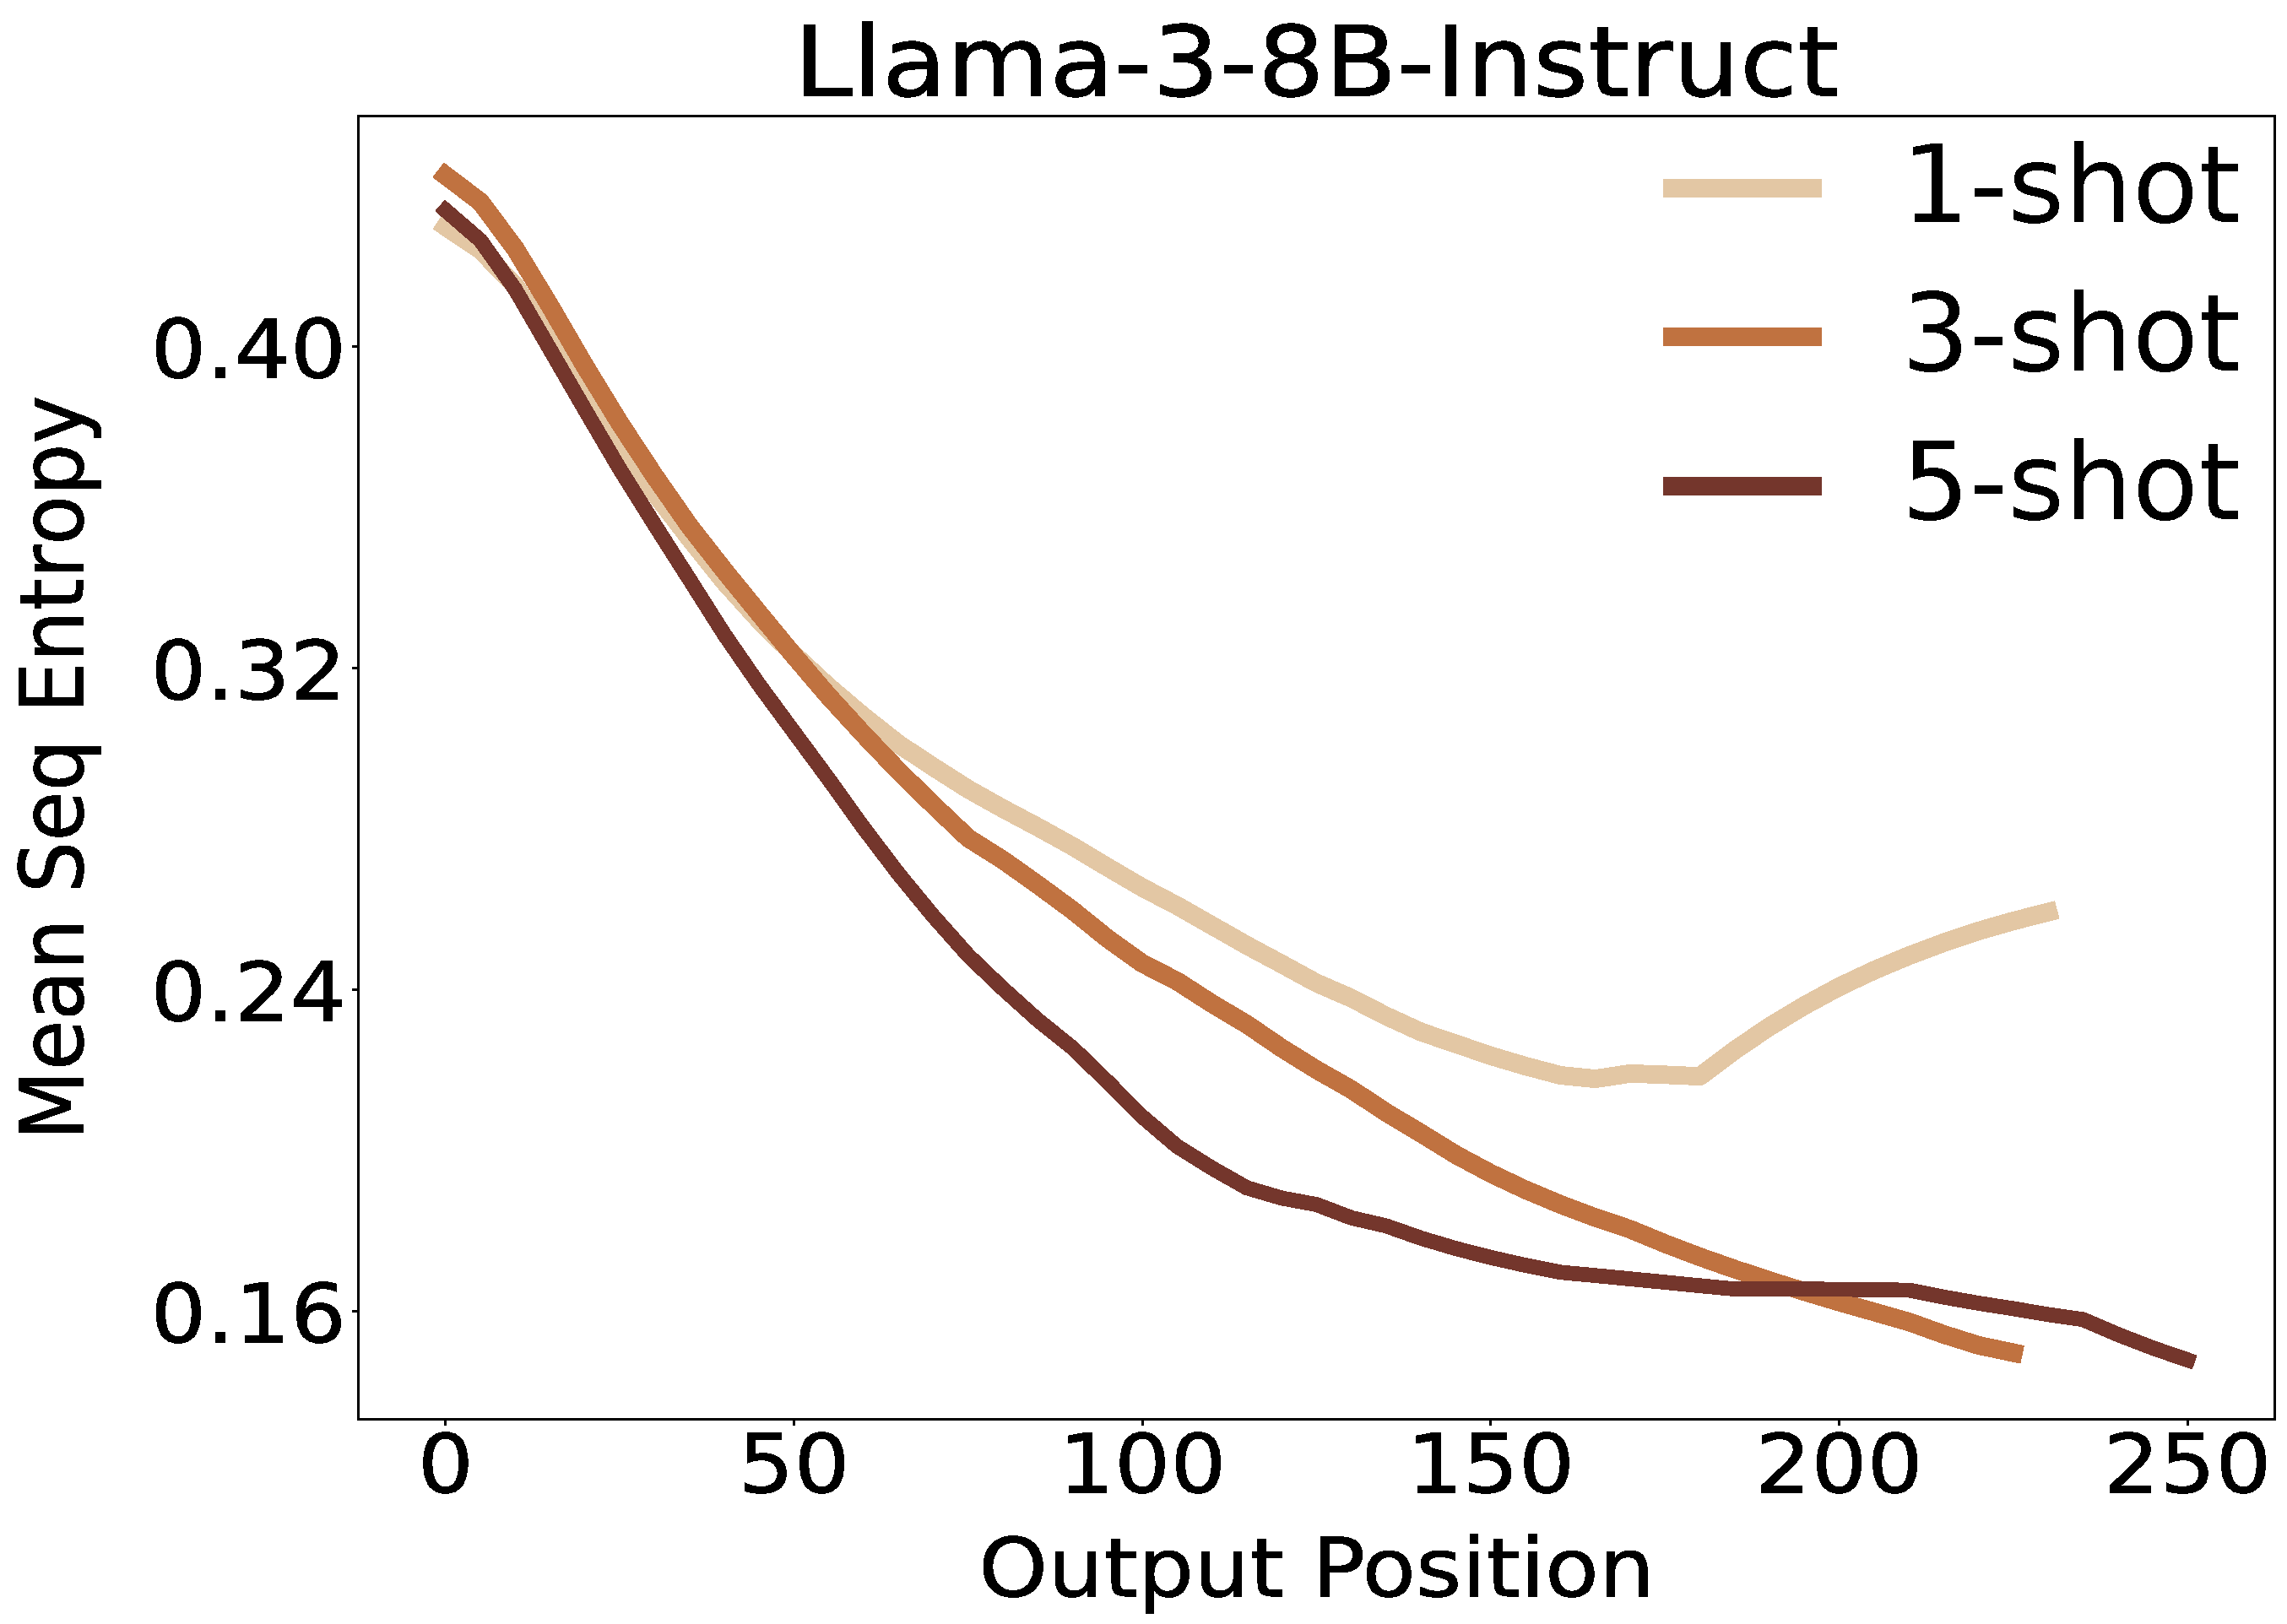
\includegraphics[width=\linewidth]{iclr2026/figures/branching_factor_figure/piecewise_ebf_Llama-3-8B-Instruct_mean_seq_entropy_fixed_start.pdf}
%     \vspace{-5mm}
%     \caption{
%     Entropy dynamics for Llama-3-8B-Instruct on the MMLU dataset. }
%     \vspace{-0.05in}
%     \label{fig: entropy_sequential_dynamic}
% \end{wrapfigure}
% We empirically validate this position-wise entropy trend on the MMLU dataset~\citep{hendrycks2021measuring}\footnote{We use MMLU as a held-out dataset with Chain-of-Thought prompting~\citep{wei2022chain} to incentivize longer reasoning outputs, aligning with a typical RLVR scenario.} using Llama-3-8B-Instruct~\citep{grattafiori2024llama}, as illustrated in \cref{fig: entropy_sequential_dynamic}.

% This trend is not merely an artifact of RL training but reflects a fundamental property known as \textit{LLM probability concentration}, where the next-token distribution naturally sharpens as generation progresses~\citep{yang2025alignment}. Indeed, research on inference-time decoding has similarly found that forcing exploration late in the sequence degrades performance by injecting low-quality outputs~\citep{liao2025lost, fu2025deep}. The well-documented continuity between base and RL-tuned models~\citep{yue2025does, zhao2025echo} indicates this principle holds true for RLVR as well, suggesting that an effective strategy must not only explore high-entropy areas, but also fruitful ones.

% These converging lines of evidence provide a clear guide for applying a classic RL principle: agents should increase exploration in states of high uncertainty~\citep{ziebart2008maximum, schulman2017equivalence, haarnoja2018soft}. By aligning our strategy with the natural dynamics of generation, we arrive at a simple yet powerful design principle: \textbf{explore early and exploit late}. This involves encouraging strong exploration when the generative trajectory is wide and gradually shifting toward exploitation as it narrows. In the next section, we will introduce a concrete method that instantiates this principle.